\chapter{結果と考察}
共振周波数を変化させるためには、共振器の大きさを変化させる方法と、と内部に誘電体あるいは導体を挿入する方法がある。共振器自体の大きさを変化させて共振周波数を調整する方法では、全ての辺の長さの比を一定にしなければ、内部の電磁場分布が大きく変化してしまい、大きさの変化とともに試料設置位置も変動させる必要が出てくるが試料設置位置を動かすことは現実的ではない。また、全ての方向で大きさの比を保ちながら共振器の大きさを変化させるためにはかなり高度なギミックが必要となり、これも現実的ではない。そのため今回は内部に誘電体を挿入することによって、共振周波数を現象させるという方法で実現を目指す。


\section{誘電体挿入による影響}
まず、誘電体挿入による影響を調べるための検証を行った。

\vspace{10 mm}

\begin{figure}[h]
  \begin{center}
    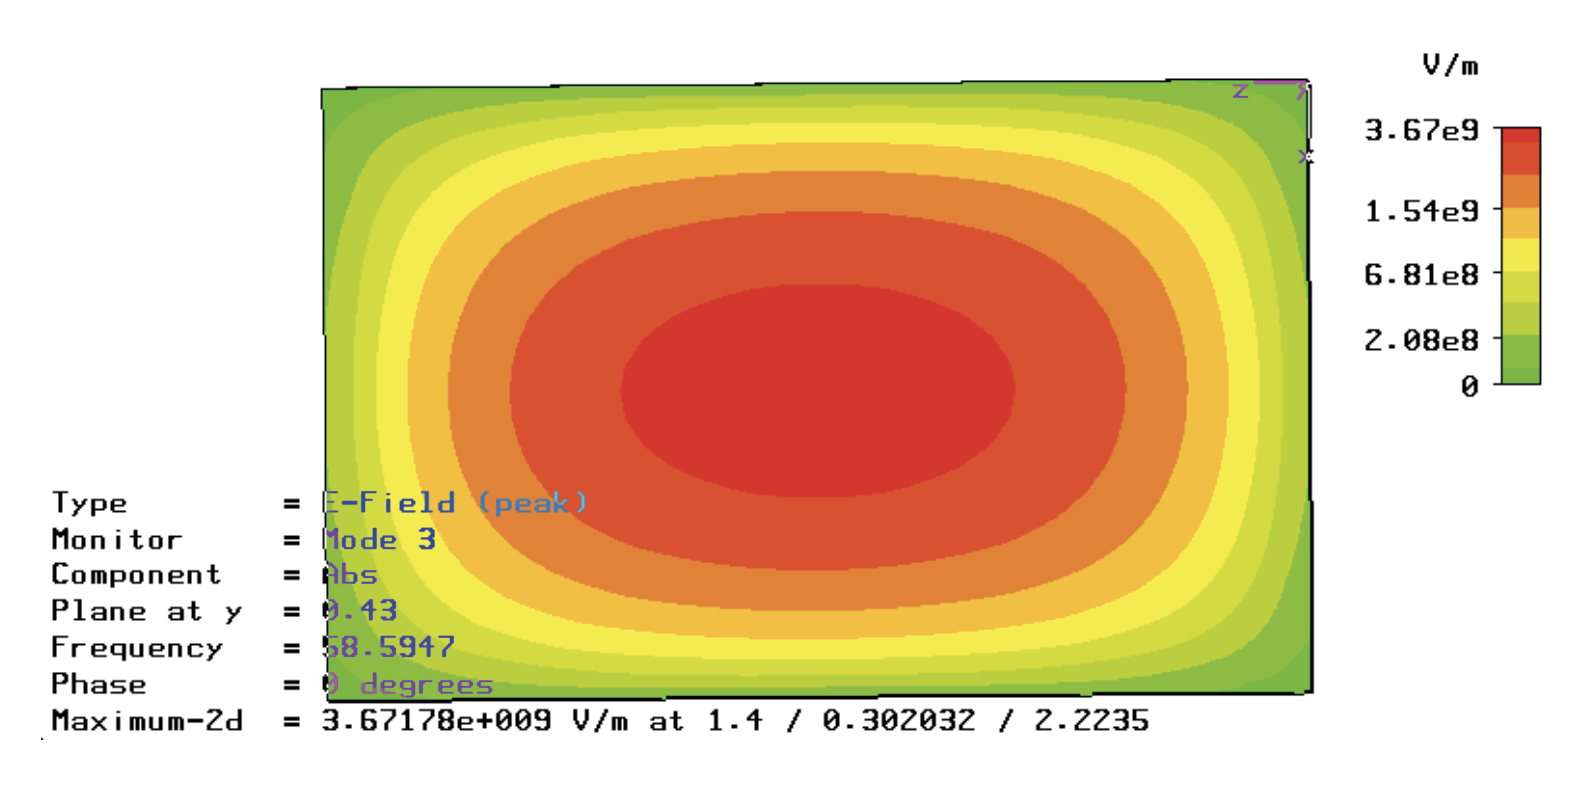
\includegraphics[width=12cm]{./image/te101.png}
    \caption{TE$_{101}$の電場分布}
    \label{fig:E-TE101}
  \end{center}
\end{figure}

図4.1 のように基本モードTE$_{101}$を持つ空洞共振器を設計した。
この図では電場分布(最大振幅)を表しており、中心の方が振幅が大きく、
端に向かうにしたがって小さくなっていることがわかる。
今回は、この共振器を用いて検証を行う。

誘電率9の誘電体(サファイア)を下図のように

\begin{enumerate}
  \item 共振器よりも小さいサイズで位置のみを変化させたモデル
  \item 共振器と同じサイズで徐々に挿入していくモデル
\end{enumerate}

の2つの場合で検証を行った。\\
水色の部分が共振器、青色の部分が誘電体(サファイア)である。
また、共振器の長さは4.8mmとし、
誘電体の位置は誘電体の初期位置でもっとも共振器中心に近い面を基準にして検証を行った。

\vspace{10 mm}

\begin{figure}[h]
  \begin{center}
    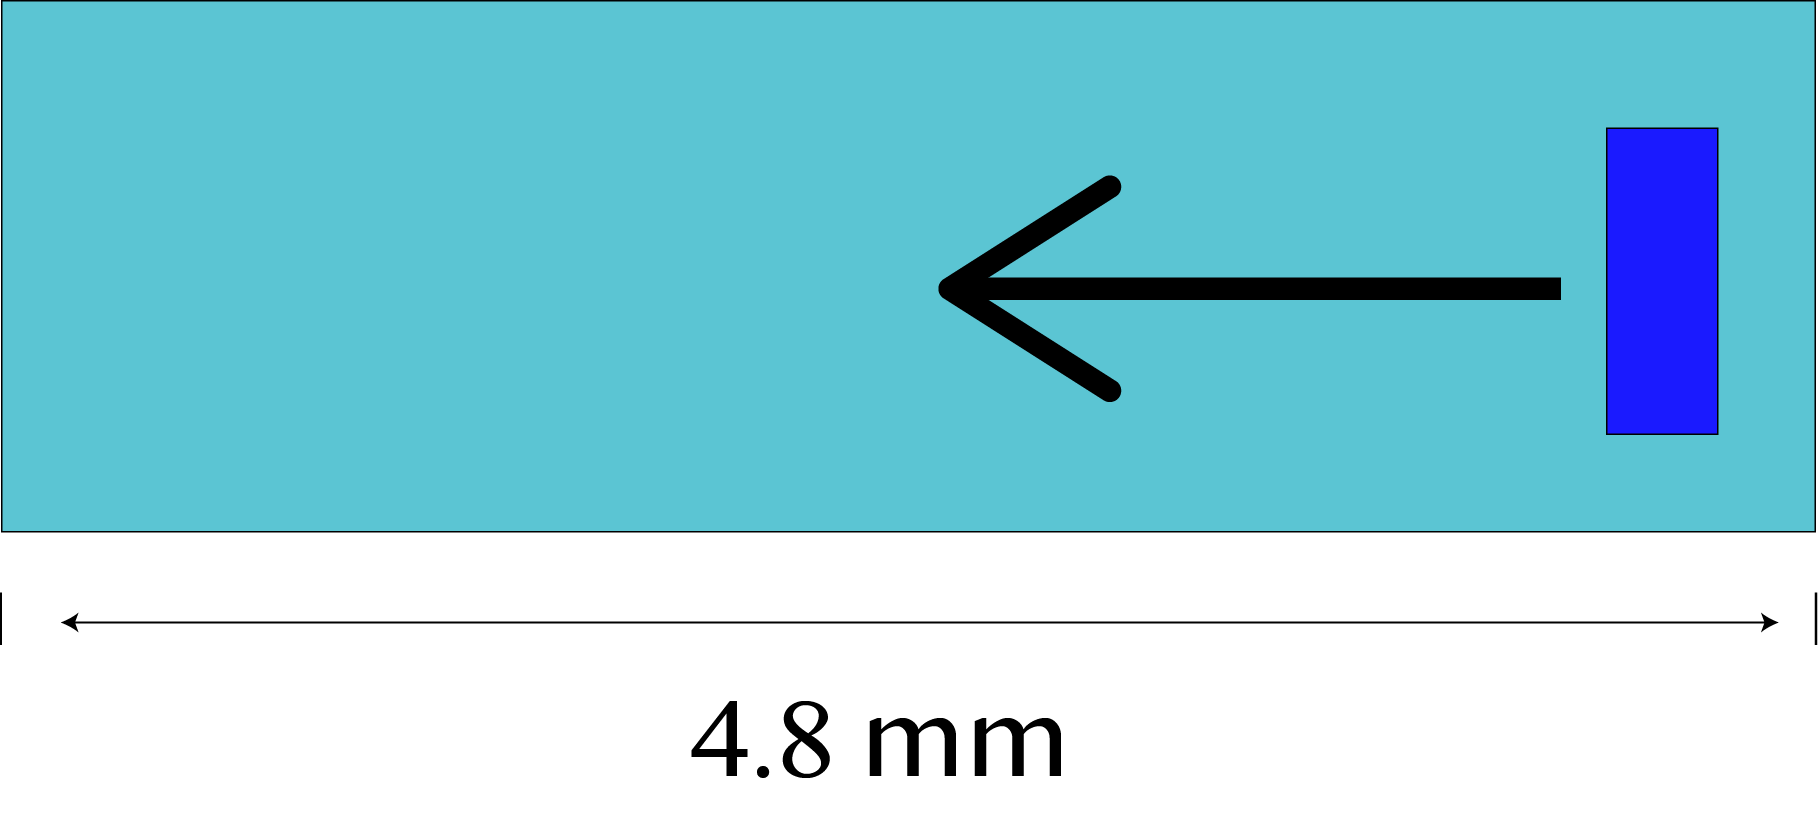
\includegraphics[width=8cm]{./image/pos.png}
    \caption{位置のみを変化させたモデル}
    \label{fig:potition}
  \end{center}
\end{figure}

\vspace{10 mm}

\begin{figure}[h]
  \begin{center}
    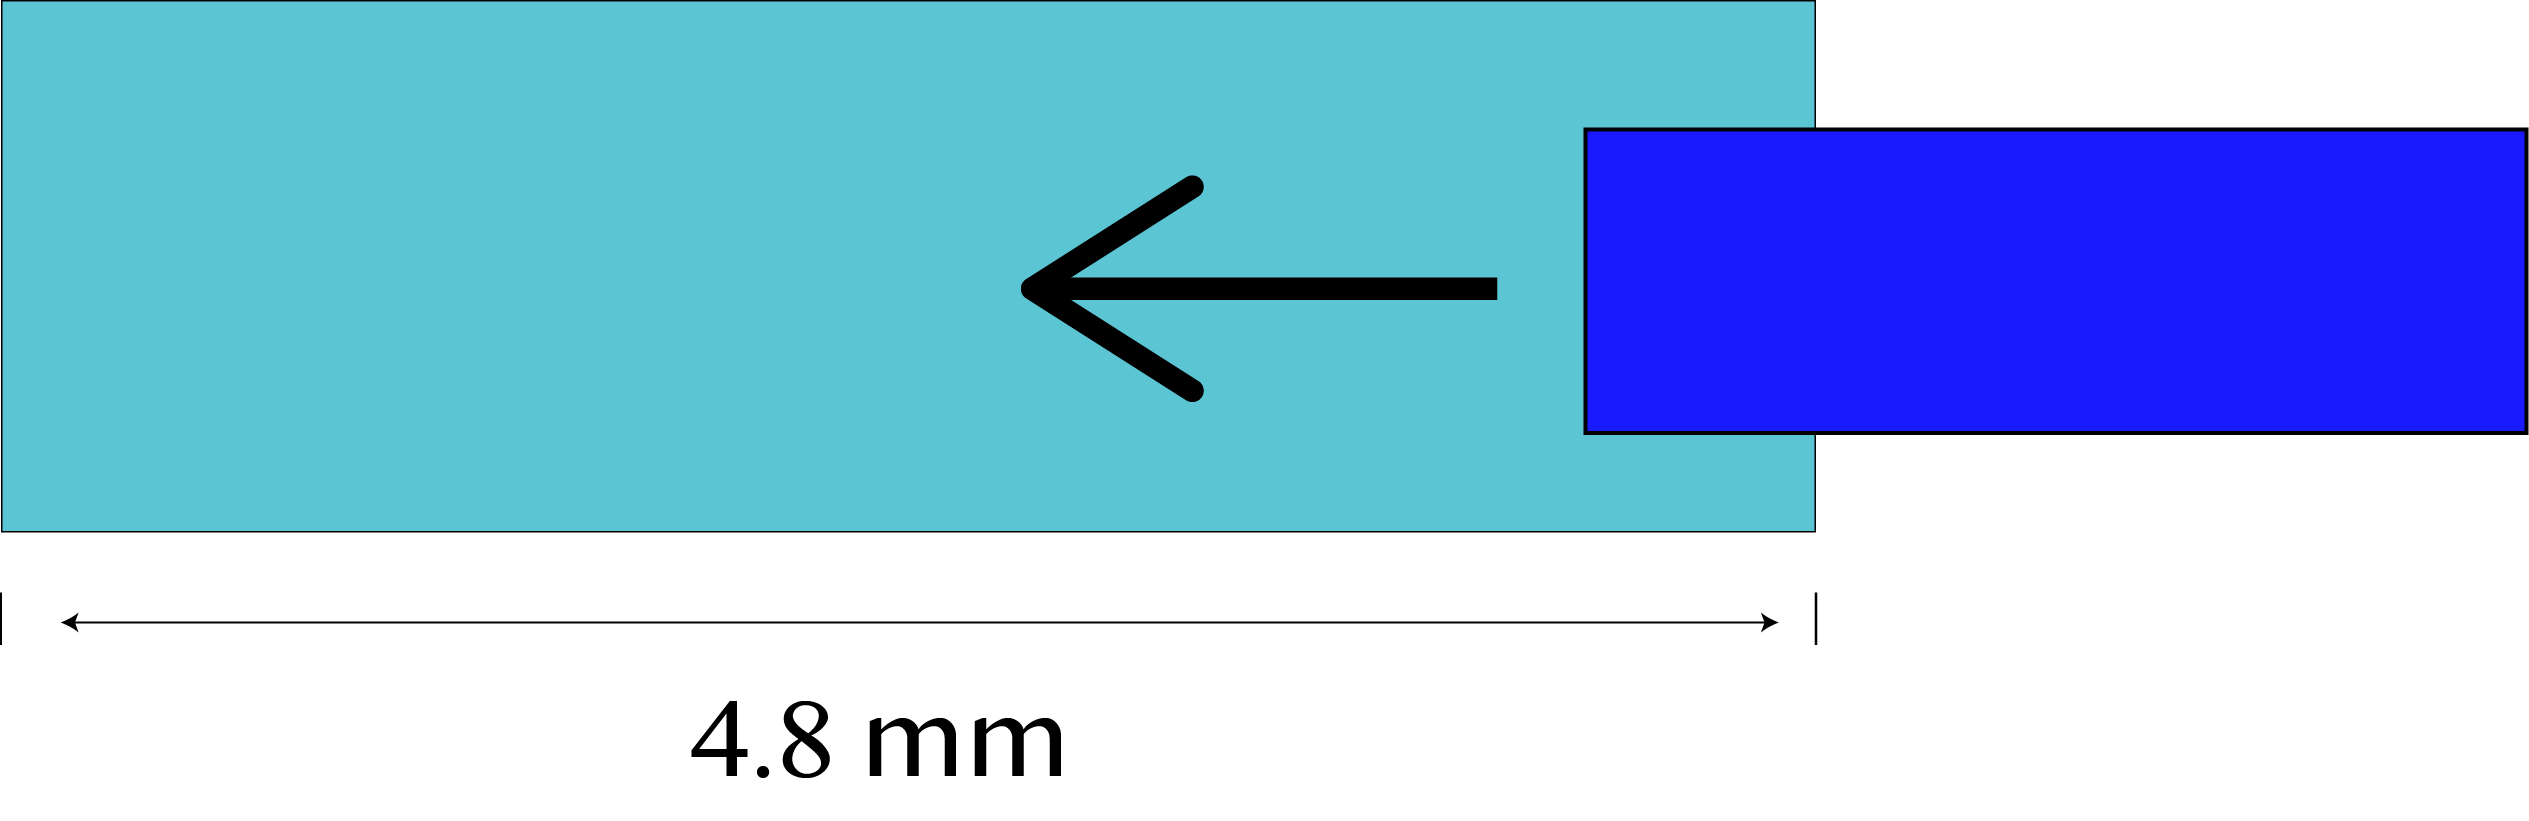
\includegraphics[width=11cm]{./image/length.png}
    \caption{誘電体を挿入していったモデル}
    \label{fig:length}
  \end{center}
\end{figure}

\subsection*{結果}
結果を以下のグラフに示す。
赤で示した点が位置のみを動かしたモデルの結果であり、青で示した点が挿入長を変化させたモデルの結果である。

この結果から、電場振幅の大きい場所に誘電体をおいた方が振幅が小さい場所におくよりも大きく共振周波数が変化すること。また、誘電体の位置だけを変化させる場合と挿入する場合では、変化の最大値は挿入していったモデルの方が大きいということがわかった。

また、どちらも一定の位置まで共振周波数が変化しなかったことから、共振の振幅が小さな場所に誘電体を挿入しても共振周波数には変化を及ぼさないということがわかった。

位置のみを変えたモデルで、共振器の末端に誘電体が到達した点の共振周波数が最初の位置での共振周波数から下がってしまっている。また、その他の点でも中心点から対照的なプロットになっていないように見える。この点については以下で考察を行う。

\vspace{10 mm}

\begin{figure}[h]
  \begin{center}
    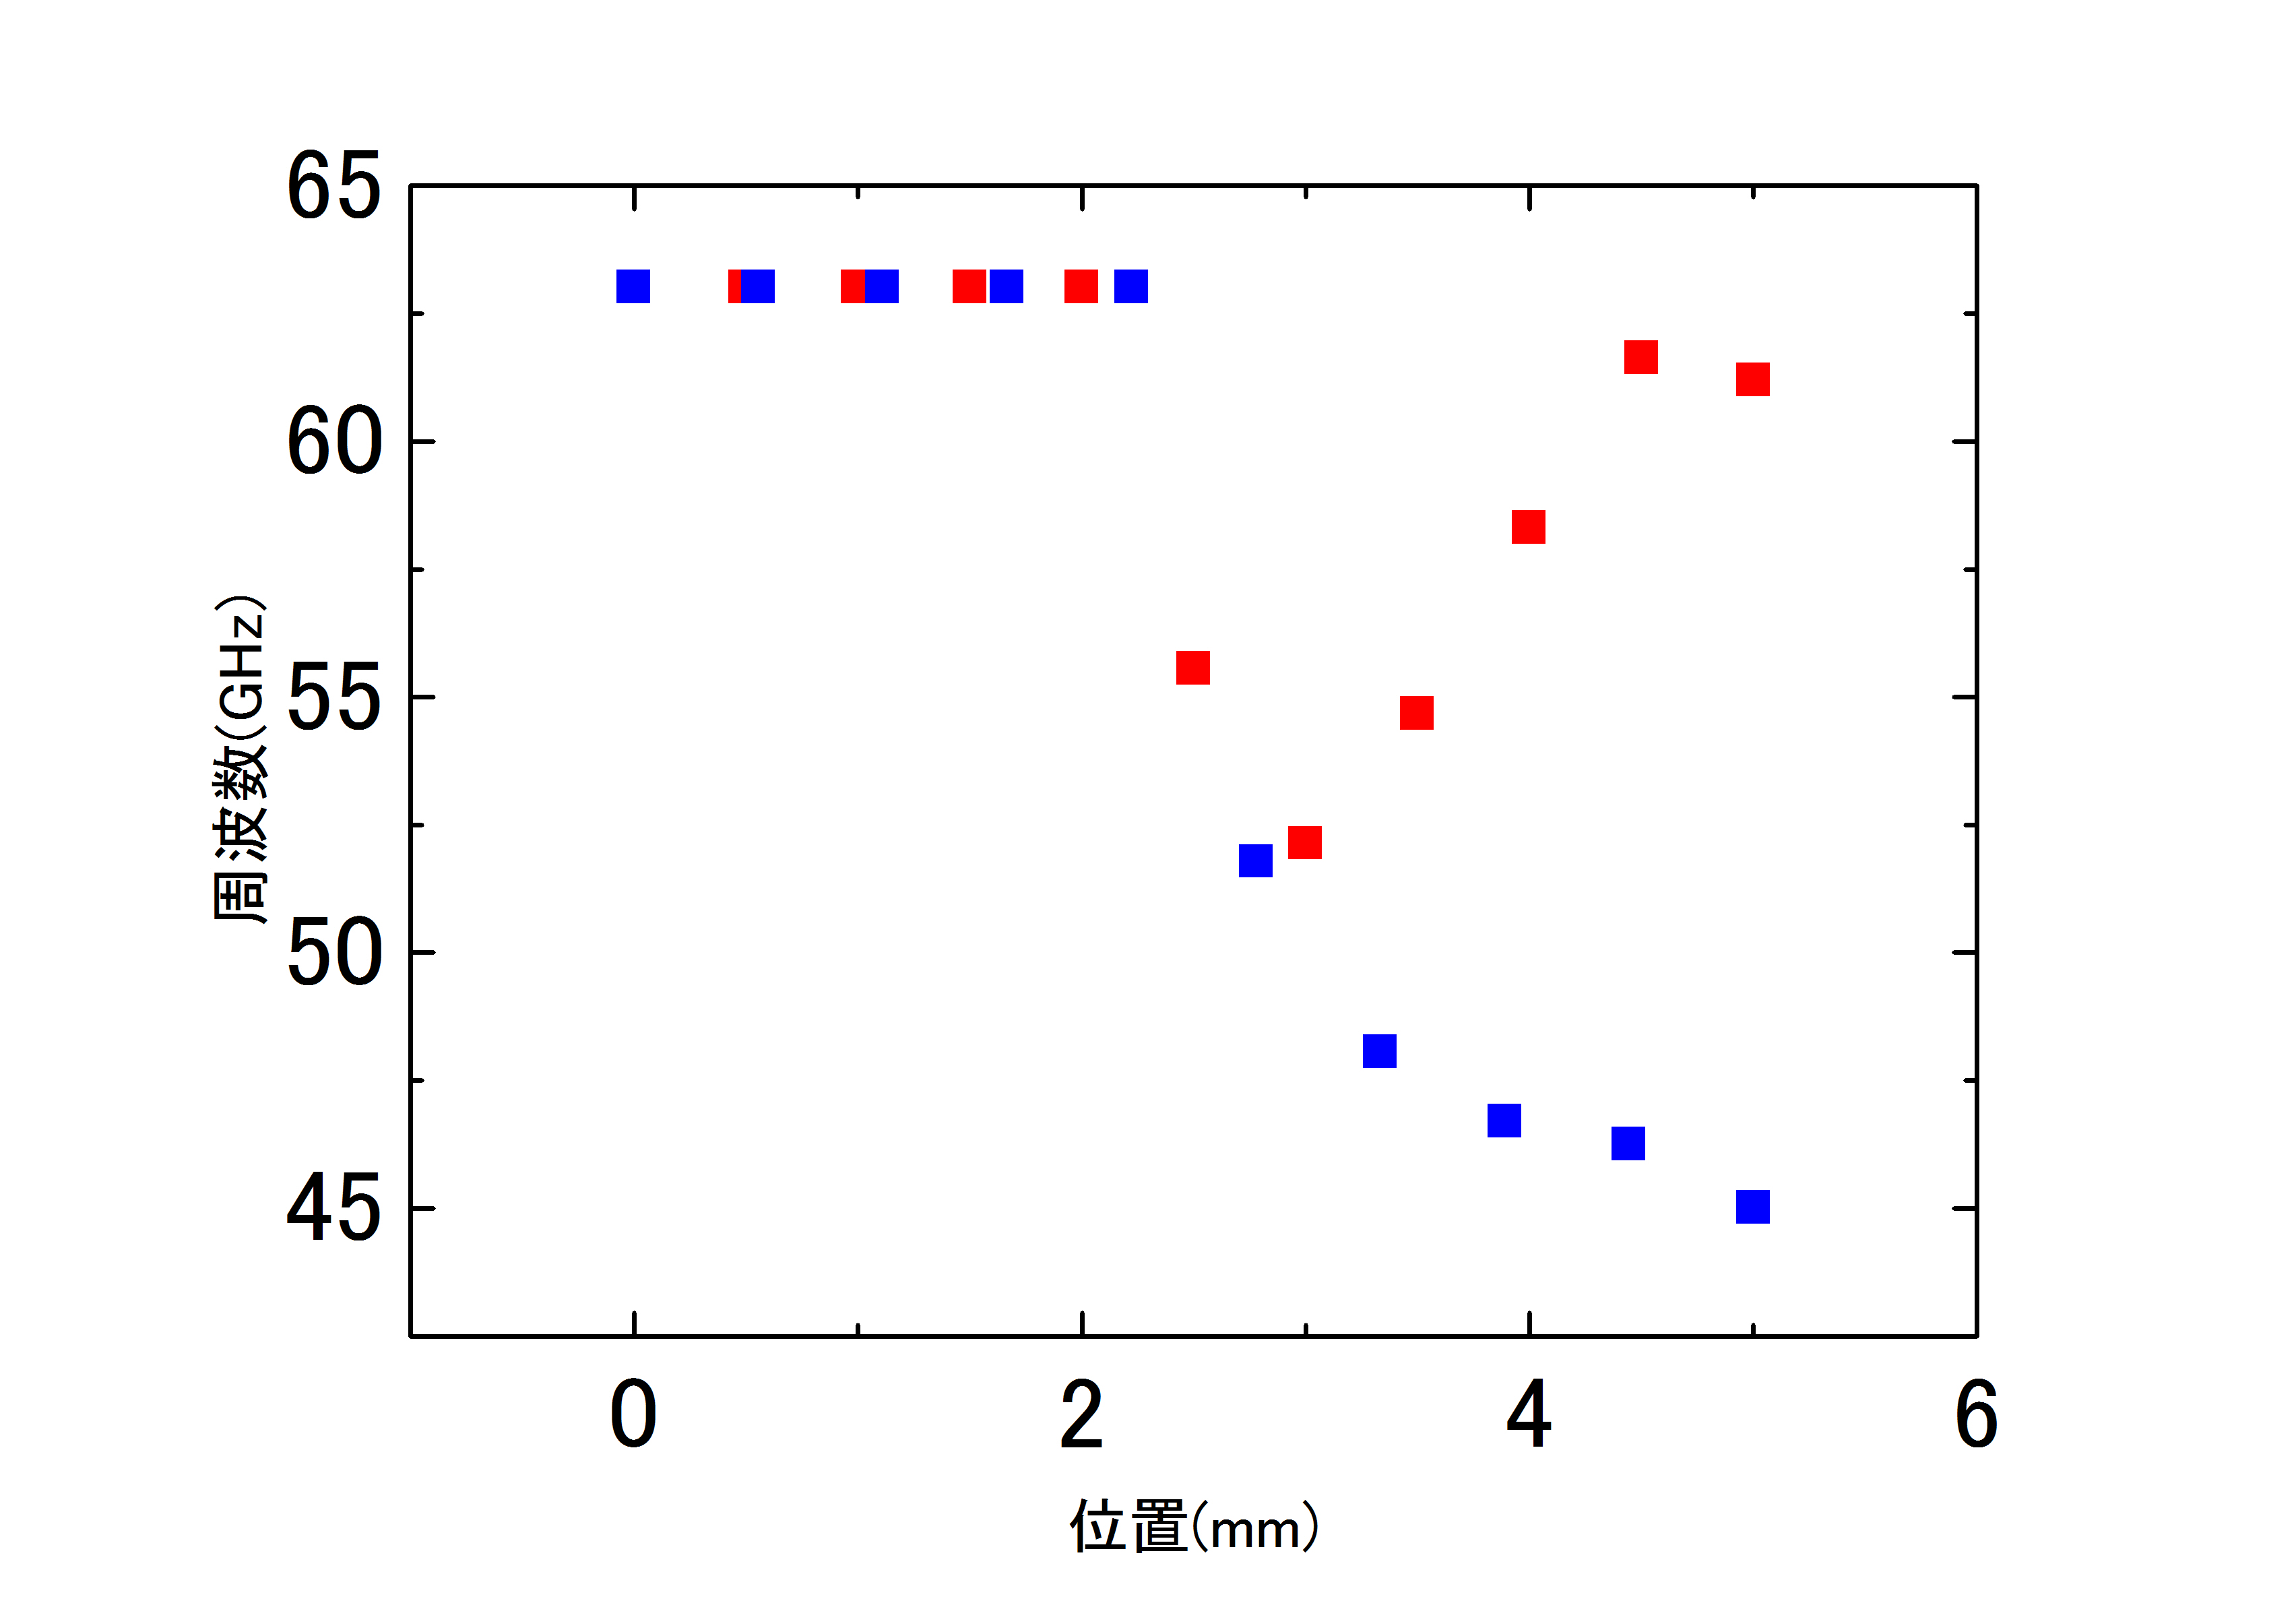
\includegraphics[width=12cm]{./image/plot1.jpg}
    \caption{誘電体による共振周波数の変化の検証}
    \label{fig:Cavity}
  \end{center}
\end{figure}


\subsection*{考察}
位置のみを変えたモデルで最後の点と最初の点での共振周波数が異なっているのは、
共振器の壁に誘電体が到達してしまったことで、
別のモードが発現し、その共振周波数が記録されてしまっているためであると考えられる。

また、対照的なプロットにならなかったのは、
位置座標の取り方が大きく影響していると考えられる。
上記の結果から、誘電体が電場振幅の強い部分に存在する際に、
共振周波数は大きく影響を受ける。
しかし、今回は誘電体の片面を基準にしてしまったために、位置によって、
誘電体のどの程度の部分が電場振幅が強い場所にあるのか、という情報が中心軸を境に、変わってしまった。
以降同様の検証を行う場合には、誘電体の中心を基準点としてとると
対照的なプロットが取れると期待出来る。



これらの結果を受けて、共振周波数を大きく変化させるためには、共振器内部の「電場振幅の大きい場所」に誘電体を「挿入」すると良さそうである。

\section{設計したモデル}
この結果を受けて今回は下図(図4.5)の基本モードTE$_{101}$,f=61GHz(固有値解析)となるような直方型空洞共振器を設計した。

\subsection*{詳細設計}
具体的には、独立した3つの方向をx,y,z方向と呼ぶとする。
以下で使う長さの単位がmmである場合には省略して表記する
基本となる空洞の大きさは(x,y,x)=(2.8,1.5,4.8)である。
共振器の底中央に大きさ(x,y,z)=(2.8,0.5,1.5)の基盤を設置した。(図4.7)
また、上部中央に共振周波数を調整するための誘電体として
大きさ(x,y,z)=(2.8,0.5,1.5)で挿入した。
挿入する誘電体は比誘電率9を持つサファイアを想定した。
誘電体、基盤として用いるサファイアは、北野研究室でよく使用されるサファイア基盤の厚さが5mmであるためそこから切り出しやすいように今回使用する厚みも5mmとした。
試料の位置は図4.5を参照。
また基盤と周波数調整誘電体の大きさが同じなのは

試料設置位置にかかる電場を最大にするためである。
また過去に行われたcavity-QED実験\cite{cQED}を参考にして、
外界との結合のため共振器上部に高さ1mm励振部を設置した。
外部との結合に用いる同軸ケーブルのサイズは外部導体の外径$φ=2.197mm$、
内部誘電体層(テフロン)の外径$φ=1.676mm$、中心導体の外径$φ=0.511mm$とした。
また、空洞共振器の壁には完全導体(PEC)を使用し、内部は真空とした。

\vspace{10 mm}

\begin{figure}[h]
  \begin{center}
    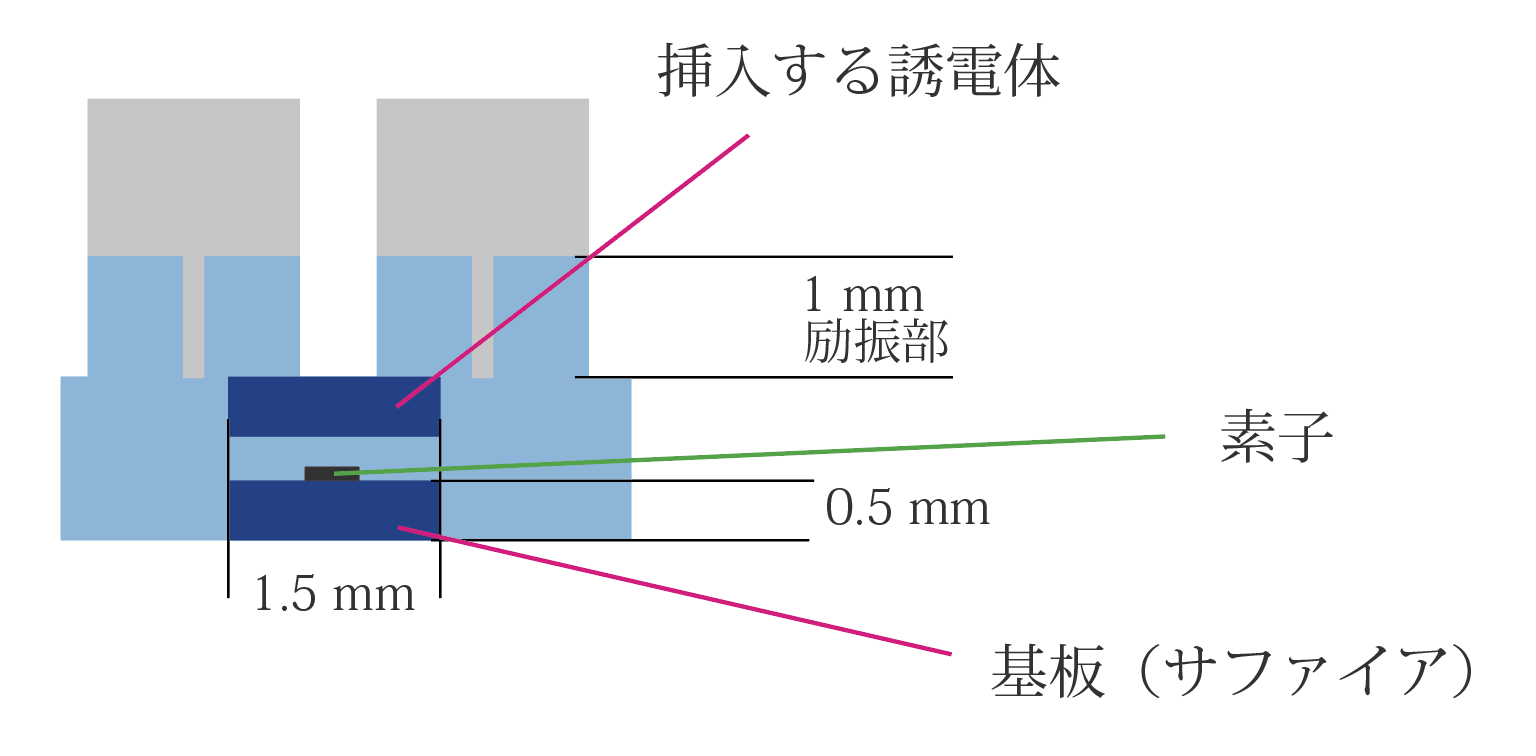
\includegraphics[width=12cm]{./image/newmodel.png}
    \caption{設計したモデルの断面からの図}
    \label{fig:Cavity}
  \end{center}
\end{figure}

\vspace{10 mm}

\begin{figure}[h]
 \begin{minipage}{0.5\hsize}
  \begin{center}
   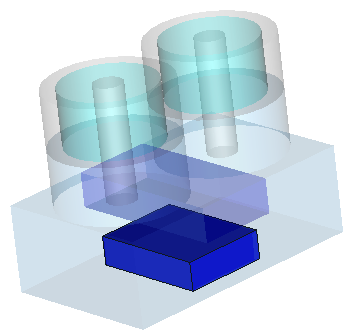
\includegraphics[width=70mm]{./image/model73.png}
  \end{center}
  \caption{設計したモデルの立体図}
  \label{fig:one}
 \end{minipage}
 \begin{minipage}{0.5\hsize}
  \begin{center}
   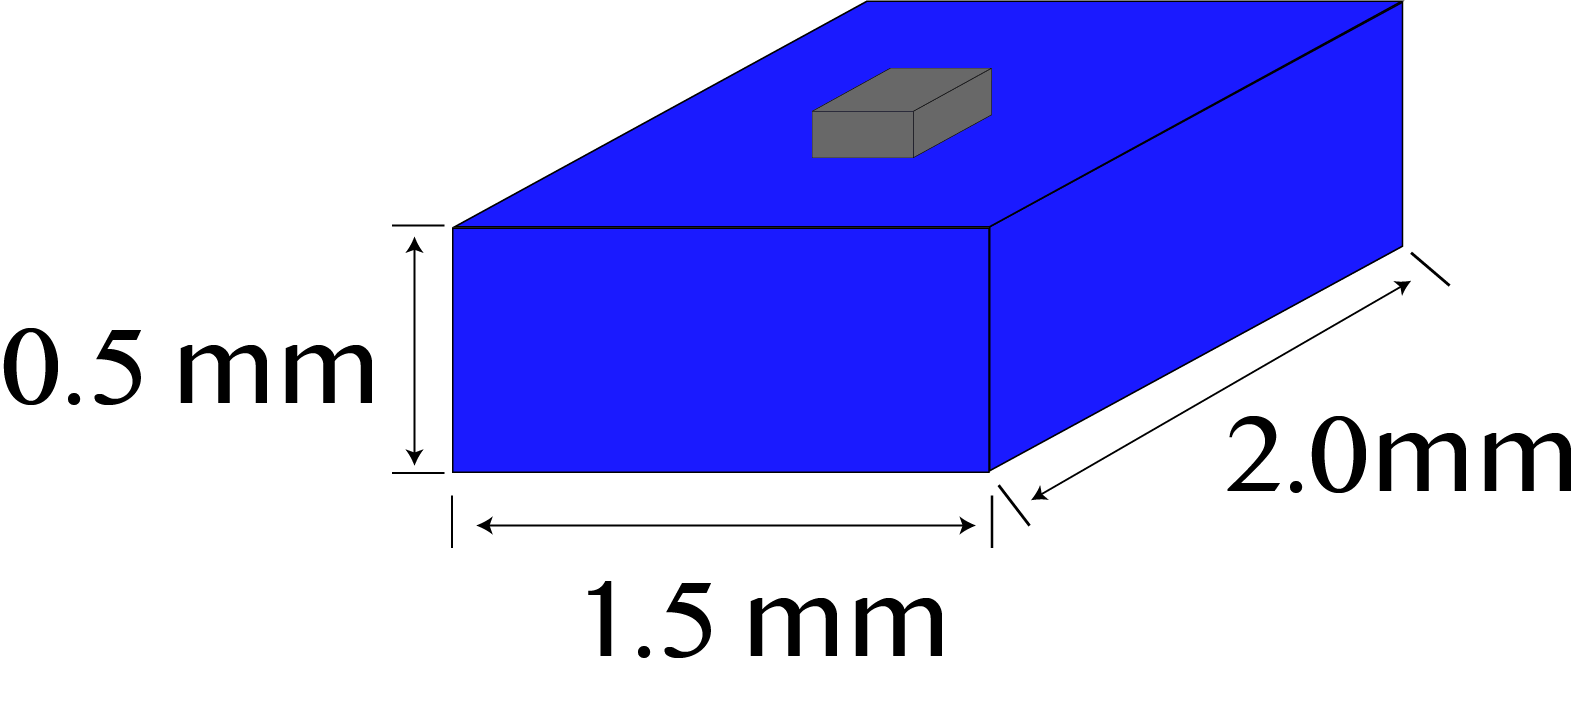
\includegraphics[width=70mm]{./image/基板資料あり.png}
  \end{center}
  \caption{基盤に試料を乗せた図}
  \label{fig:two}
 \end{minipage}
\end{figure}

実際に実験を行う際には、図4.7にあるように、
共振器の底に設置した誘電体の上には超伝導体の試料を載せる。

\subsection*{基本性質}
この共振器の基本的な性質を示す。
以下それぞれ、左に固有値解析の結果、右に過渡解析の結果を示す。
過渡解析の結果はSパラメータを表示している。
シミュレーションでは入力ポートと出力ポートを設定しており、
下図赤線で示されたS$_{11}$は入力電力に対する反射電力比を示し、
下図青線で示されたS$_{21}$は入力電力に対する透過電力比を示す。
その2つの値が大きく逆向きに変動している場所で共振していると言える。


\subsubsection{誘電体なし基盤なし}
まず誘電体も基盤も全く設置していない場合の解析結果は以下のようになっている。
過渡解析の結果、狙ったモード(TE$_{101}$)での共振も観測された。
前述の基盤や調整誘電体の場所はこの結果を受けて、決定している。

\begin{figure}[h]
 \begin{minipage}{0.5\hsize}
  \begin{center}
   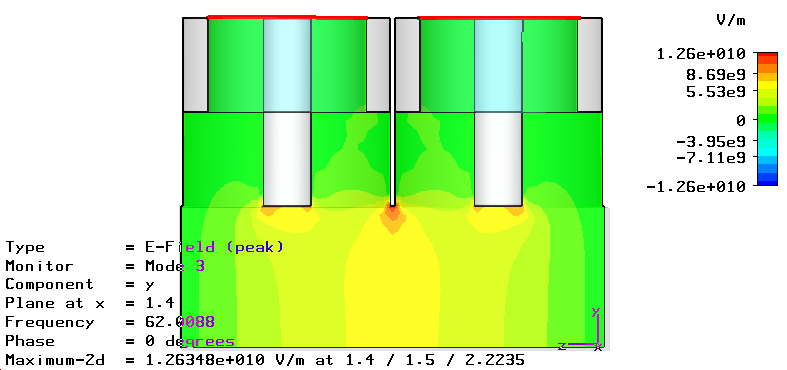
\includegraphics[width=70mm]{./image/model73_vac.png}
  \end{center}
  \caption{誘電体基盤なしy軸方向の電場分布}
  \label{fig:one}
 \end{minipage}
 \begin{minipage}{0.5\hsize}
  \begin{center}
   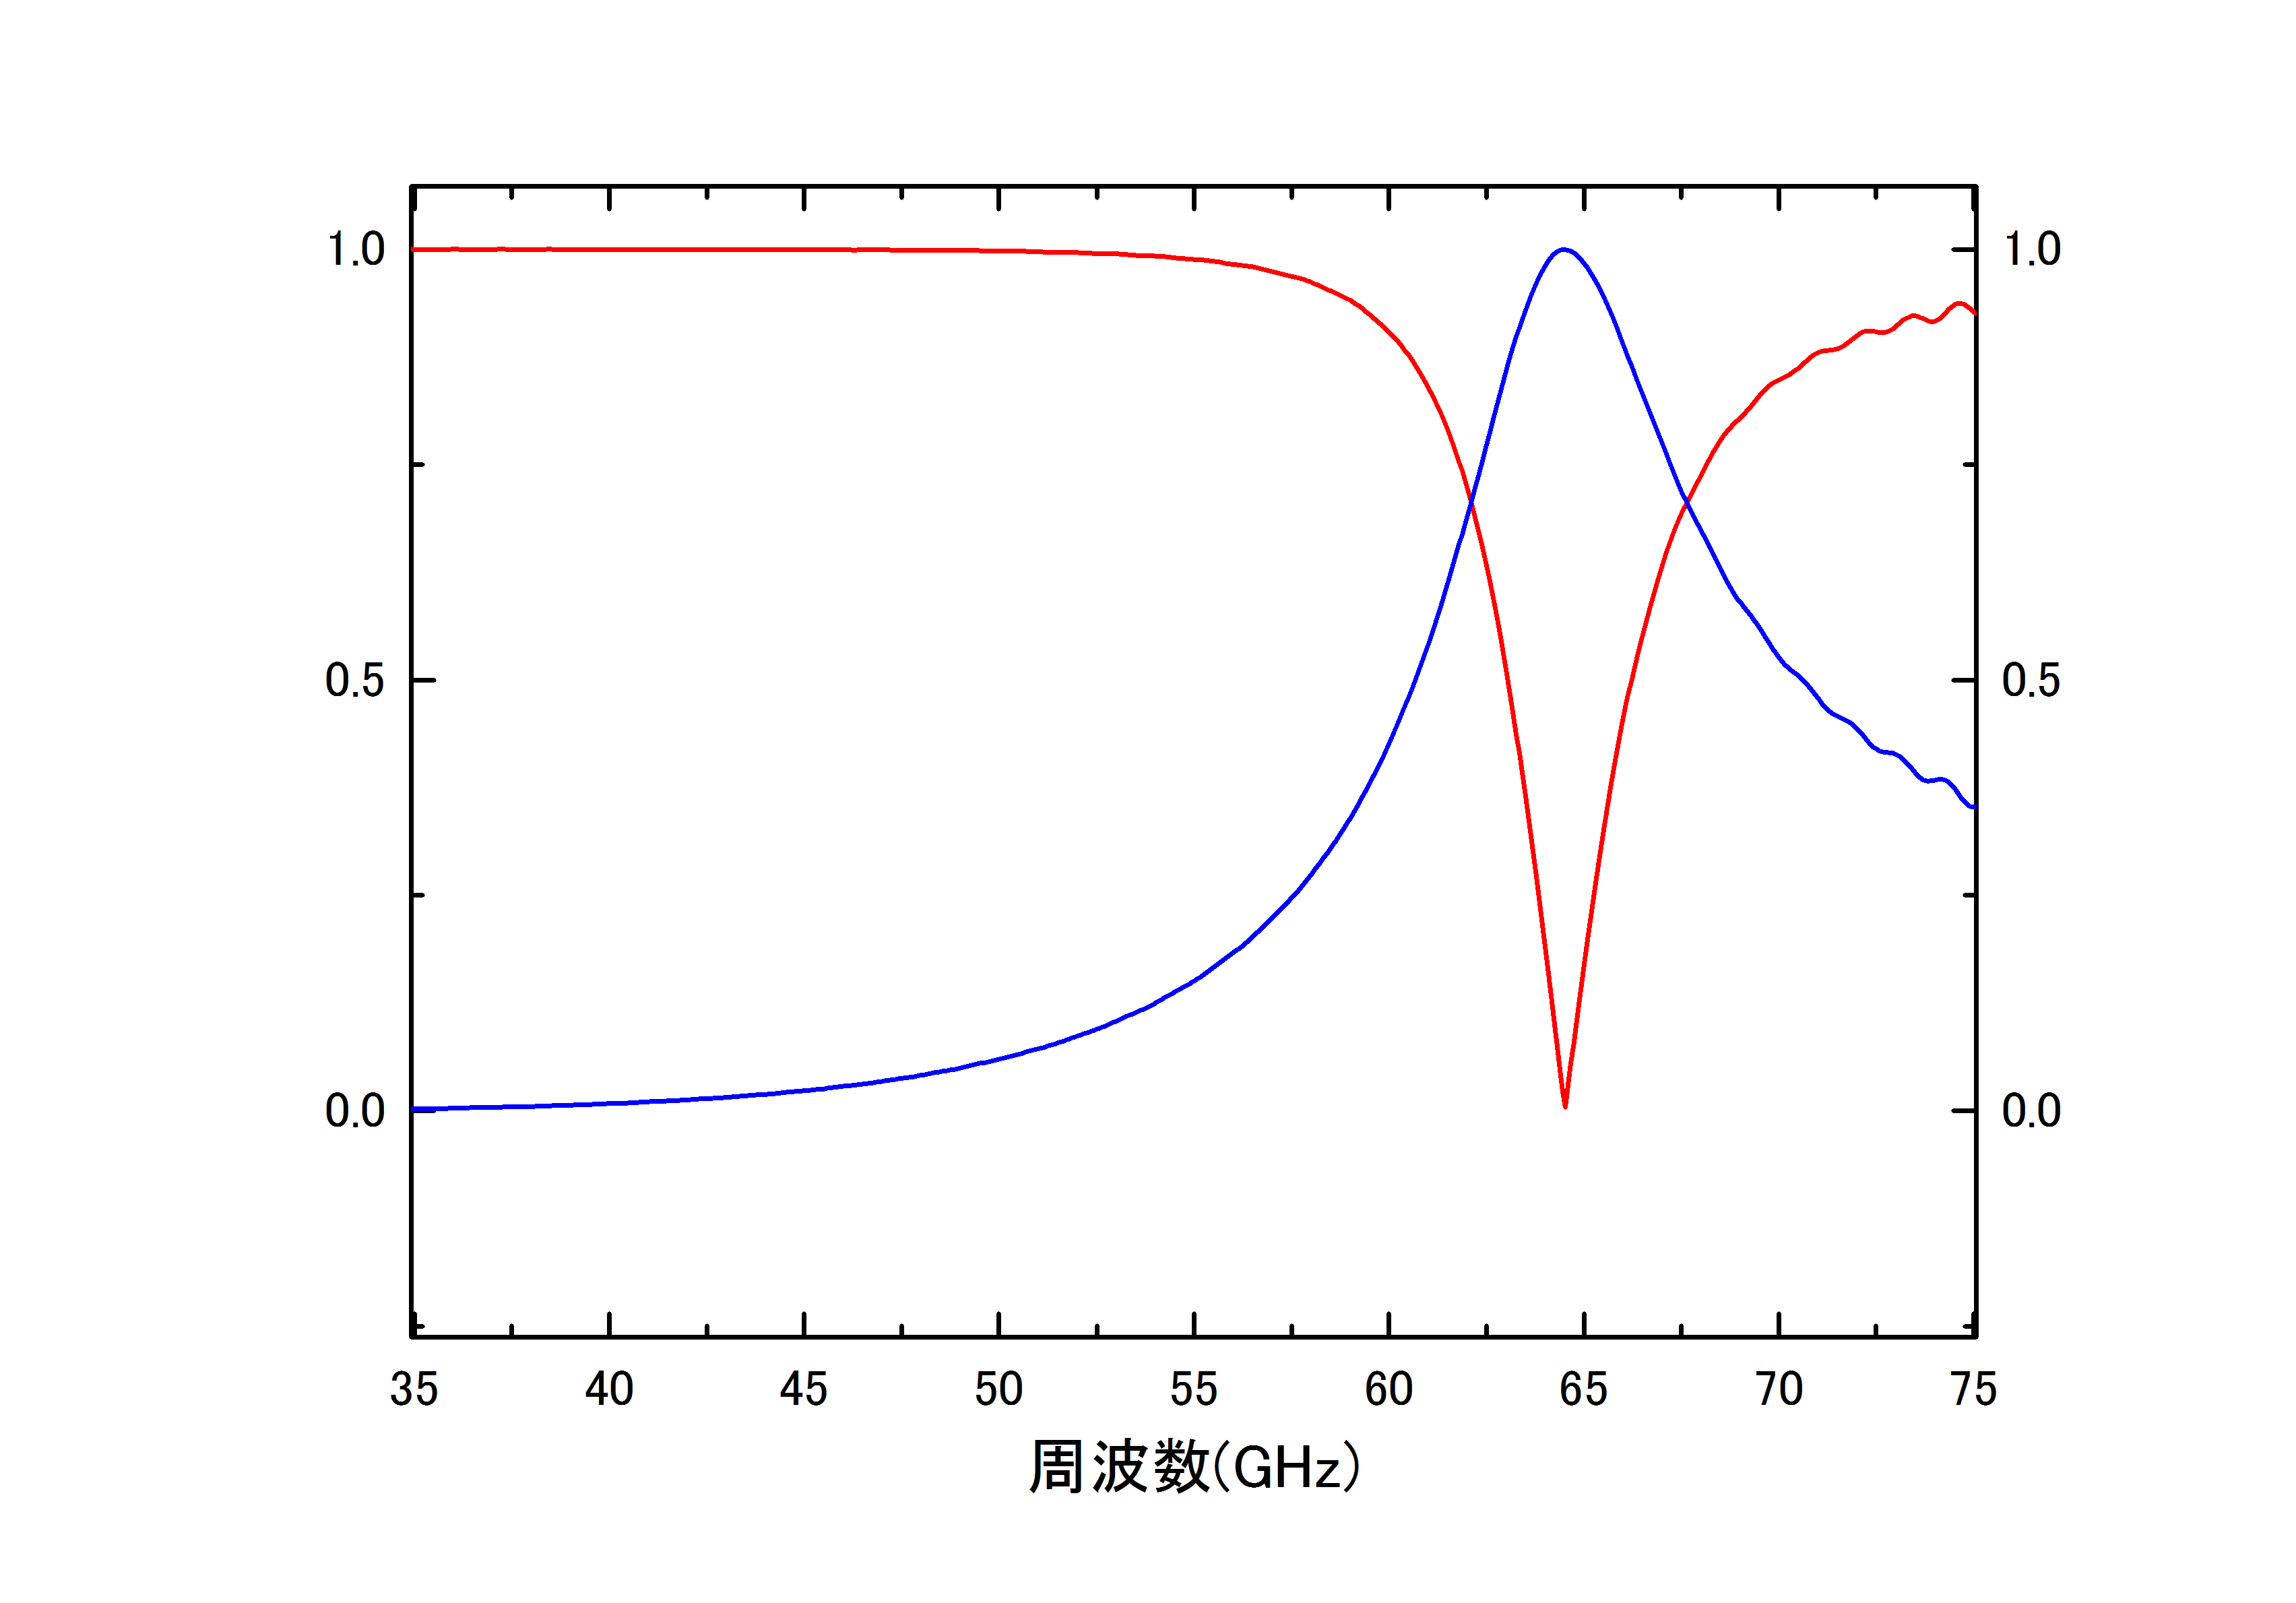
\includegraphics[width=70mm]{./image/Graph1.jpg}
  \end{center}
  \caption{誘電体基盤なしSパラメータ}
  \label{fig:two}
 \end{minipage}
\end{figure}

\subsubsection{誘電体なし基盤あり}
共振周波数を調整するための誘電体は入れずに、基盤のみ共振器内部に存在するモデルでシミュレーションを実行した。
試料が乗っている基盤は動かさないため、この値が今回得られる共振周波数の最大値となる。
基盤自体も誘電体であるため、空の場合よりも共振周波数が下がってしまっているが、
最大値として52GHz程度の共振周波数が得られそうである。


\begin{figure}[h]
 \begin{minipage}{0.5\hsize}
  \begin{center}
   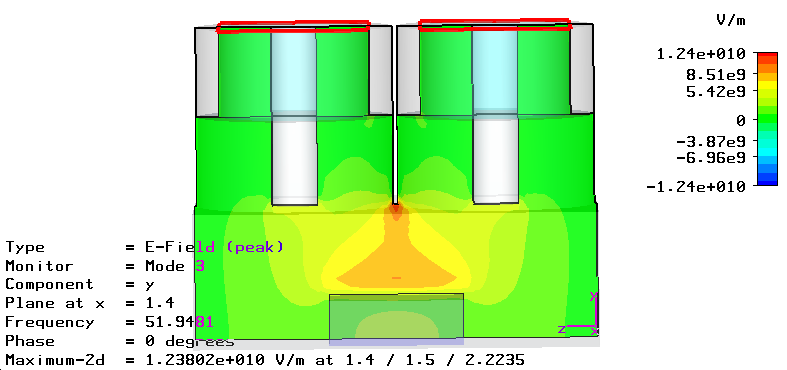
\includegraphics[width=70mm]{./image/model73_kiban_e_y_y.png}
  \end{center}
  \caption{誘電体なし基盤ありy軸方向の電場分布}
  \label{fig:one}
 \end{minipage}
 \begin{minipage}{0.5\hsize}
  \begin{center}
   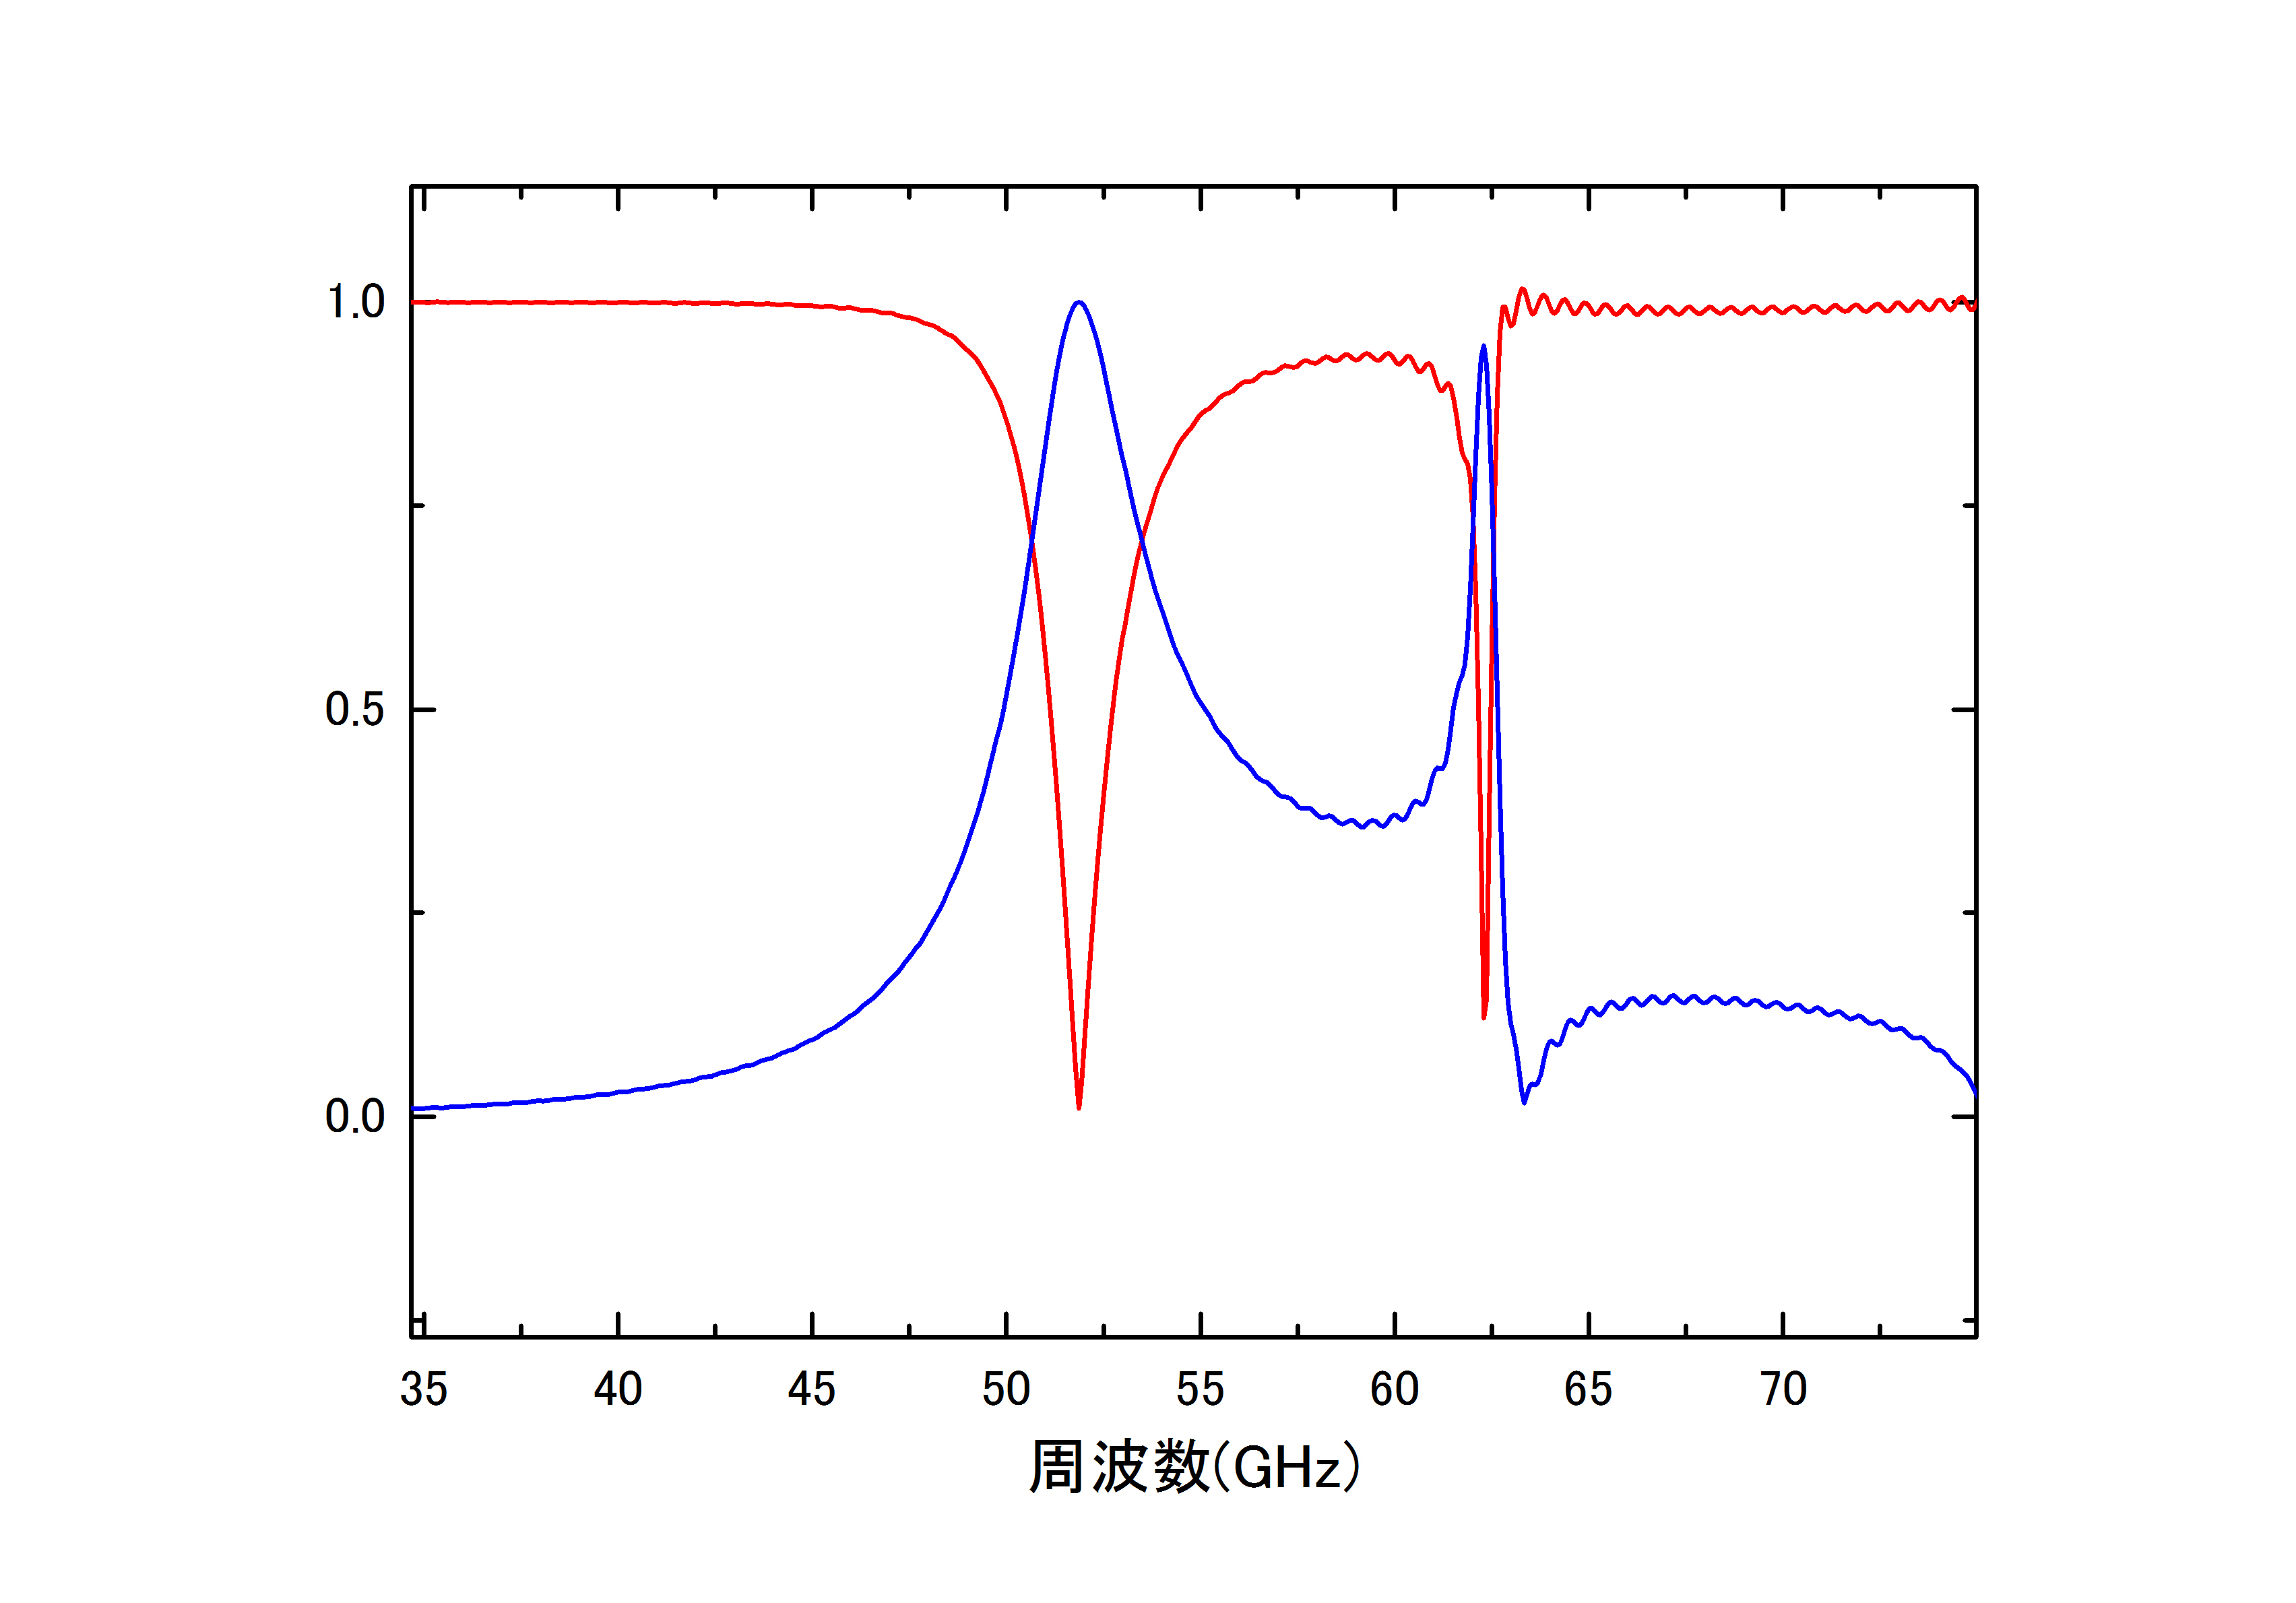
\includegraphics[width=70mm]{./image/Graph5.jpg}
  \end{center}
  \caption{誘電体なし基盤ありSパラメータ}
  \label{fig:two}
 \end{minipage}
\end{figure}

\subsubsection{誘電体あり基盤あり}
最後に共振周波数を調整するための誘電体と、
基盤をどちらも含めたモデルでシミュレーションを行った。
これが今回得られる共振周波数の最小値となる。
その結果、37GHz程度まで共振周波数を減少させることができた。

\begin{figure}[h]
 \begin{minipage}{0.5\hsize}
  \begin{center}
   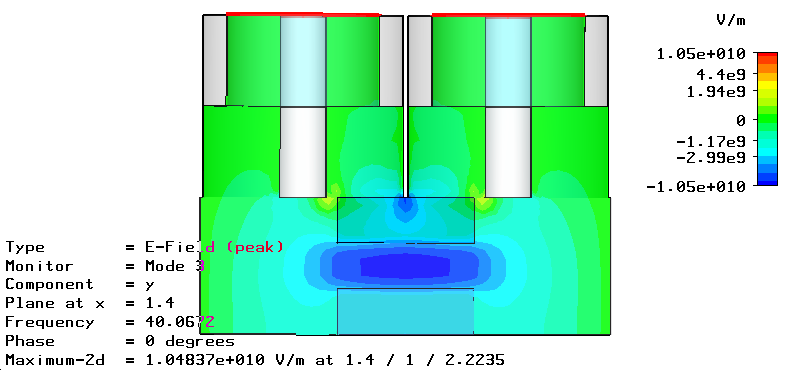
\includegraphics[width=70mm]{./image/model73_y_x.png}
  \end{center}
  \caption{誘電体基盤ありy軸方向の電場分布}
  \label{fig:one}
 \end{minipage}
 \begin{minipage}{0.5\hsize}
  \begin{center}
   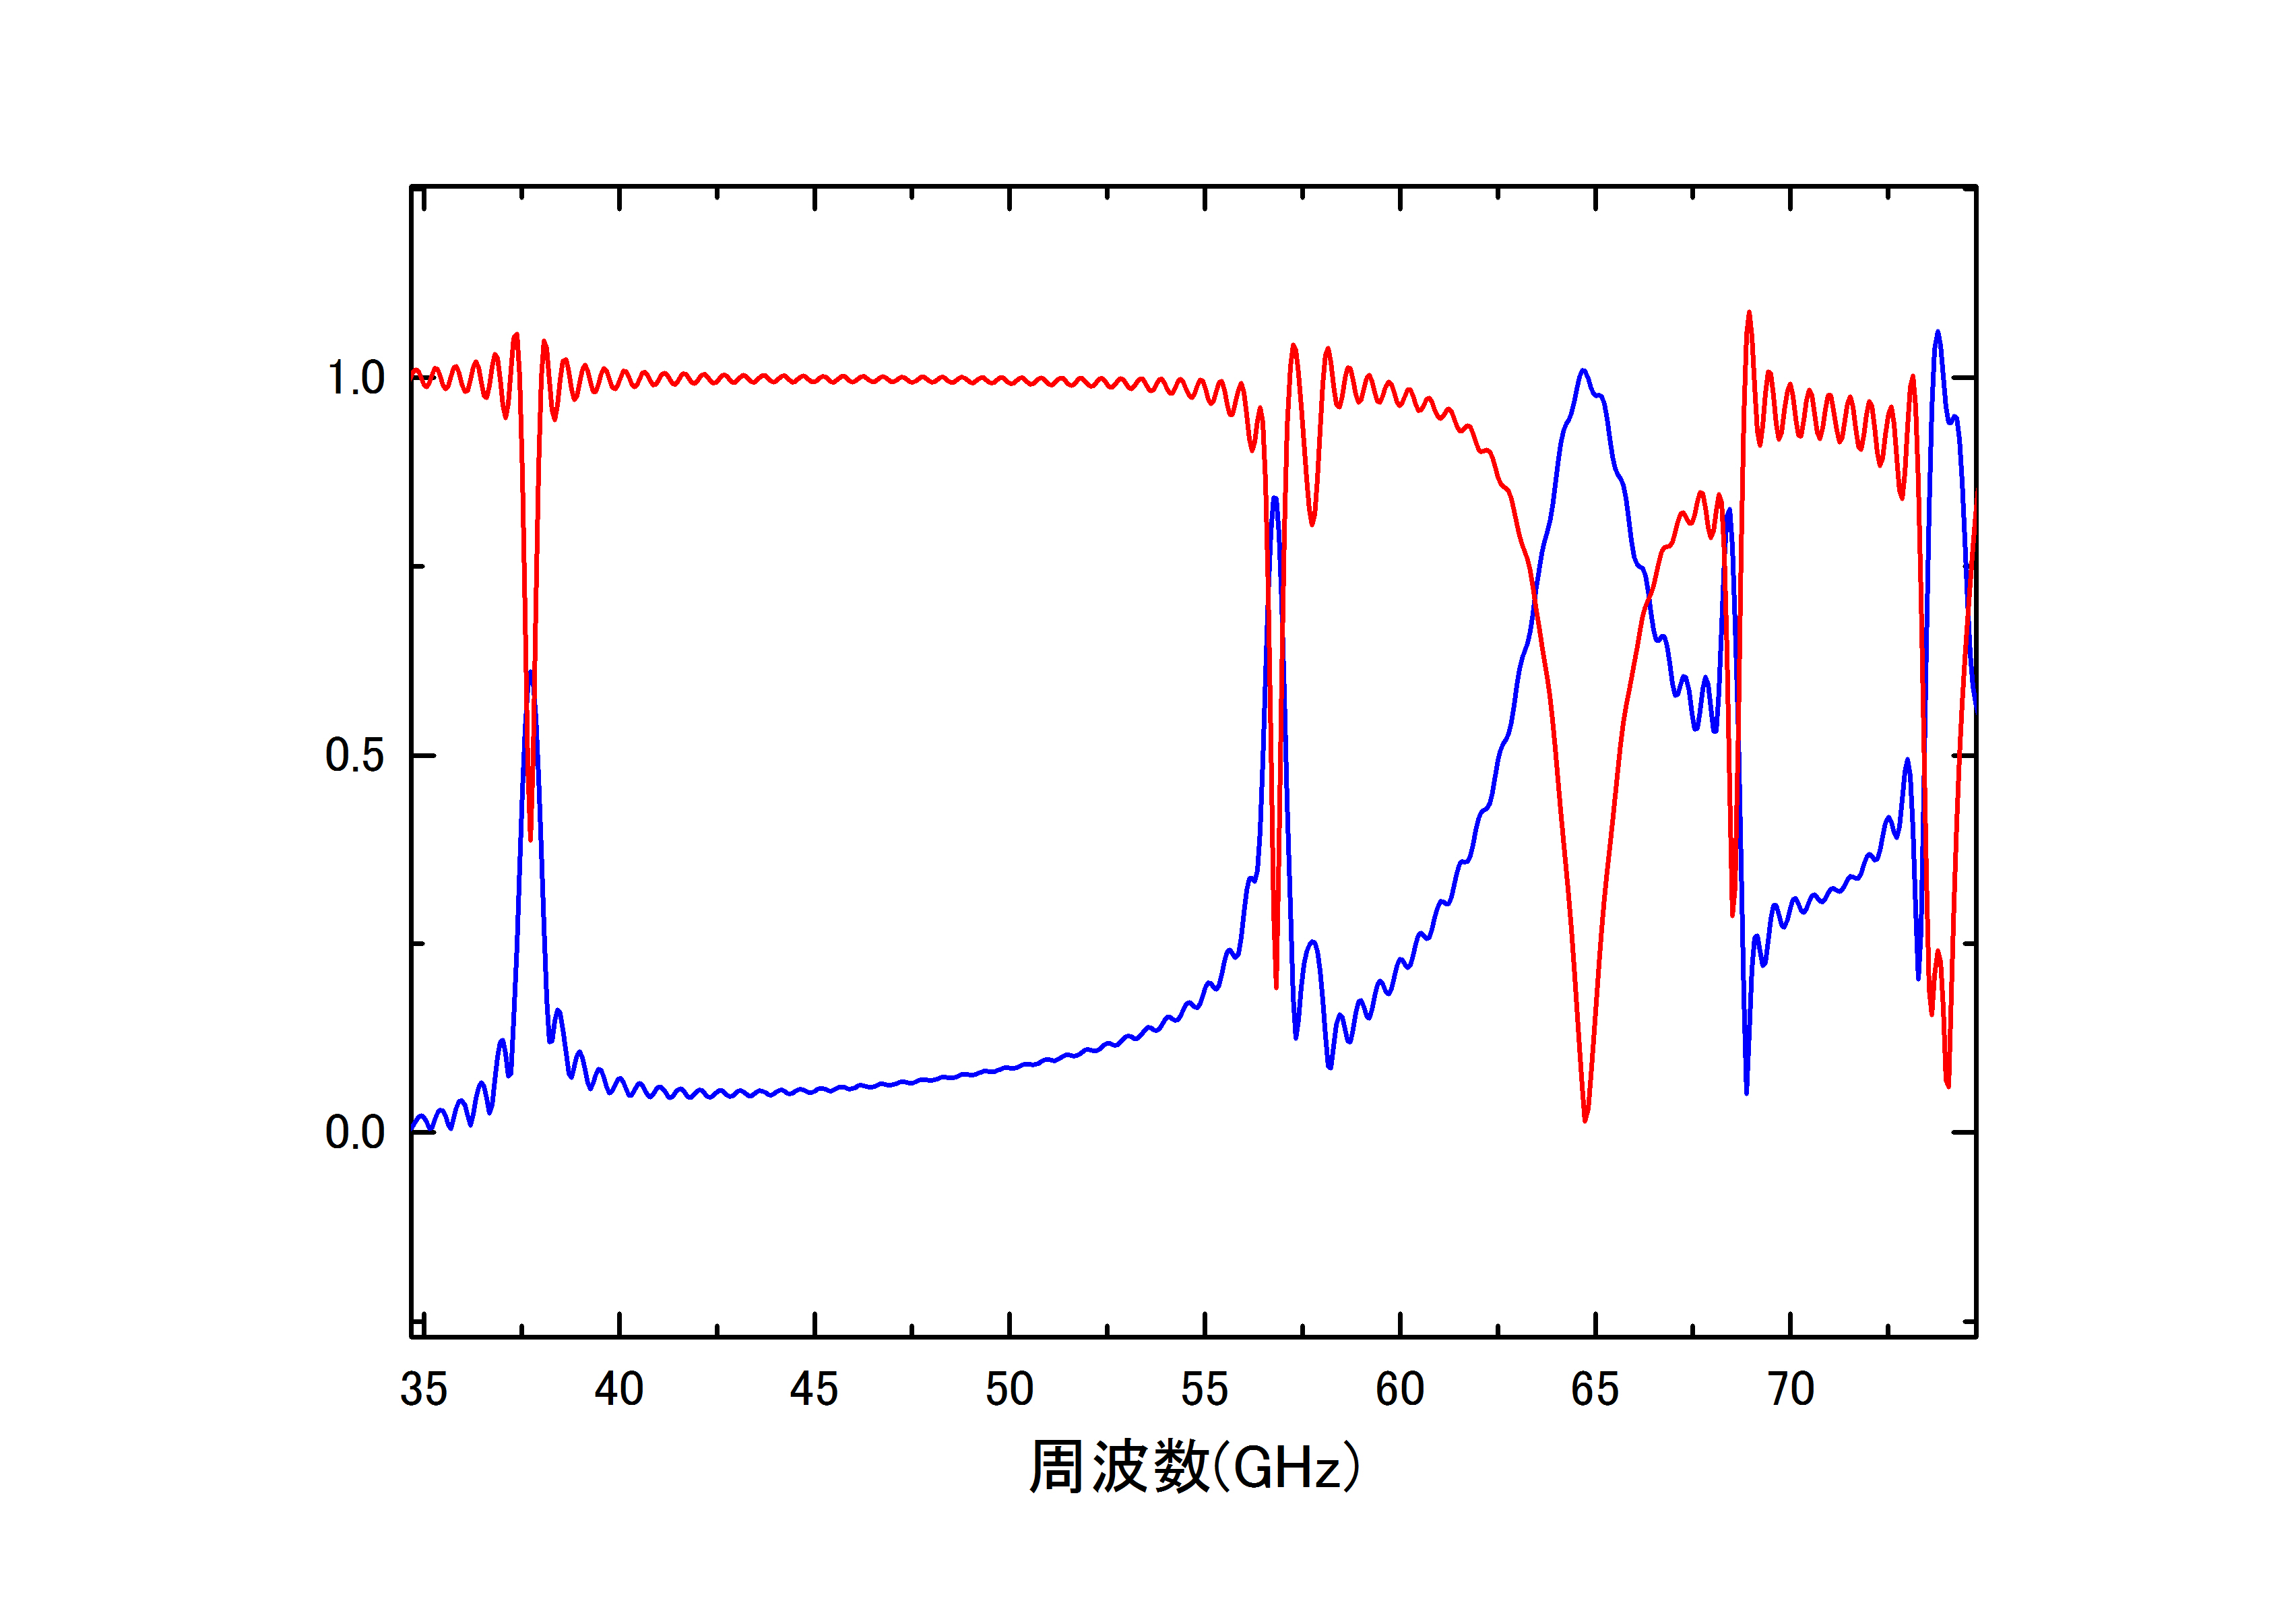
\includegraphics[width=70mm]{./image/Graph4.jpg}
  \end{center}
  \caption{誘電体基盤ありSパラメータ}
  \label{fig:two}
 \end{minipage}
\end{figure}

\subsection*{誘電体挿入時の共振周波数変化}
次に、図4.14のように誘電体を徐々に共振器内部へ挿入していった場合の共振周波数の変化を
過渡解析で検証した。
なお、水色の部分が共振器、青色の部分が誘電体である。
同軸ケーブルは省略している。
\vspace{10 mm}

\begin{figure}[h]
  \begin{center}
    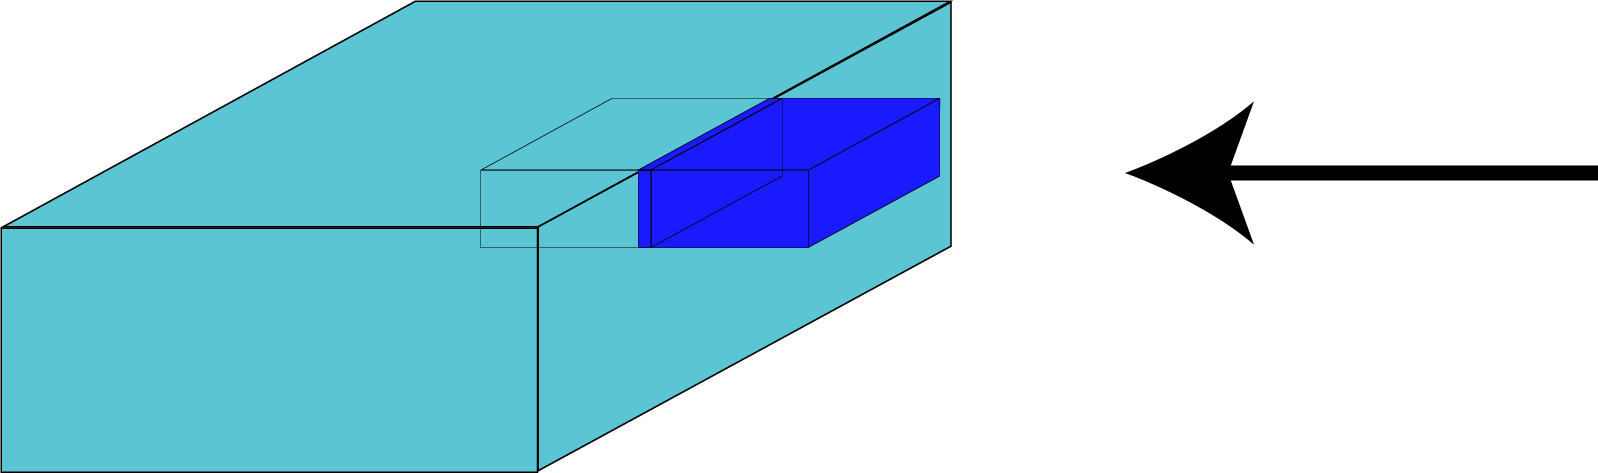
\includegraphics[width=8cm]{./image/insert.png}
    \caption{共振器への誘電体挿入}
    \label{fig:insert}
  \end{center}
\end{figure}

解析結果を図4.15に示す。
誘電体挿入と共に固有モードの数が変わってしまい、モードを共振周波数の低い順に、順番で判断する固有値解析モードでは様々なモードが混じってしまうため、
今回は過渡解析の結果を利用した。
その結果から共振ピークと判断出来る点を取り出し、プロットした。

\vspace{10 mm}

\begin{figure}[h]
  \begin{center}
    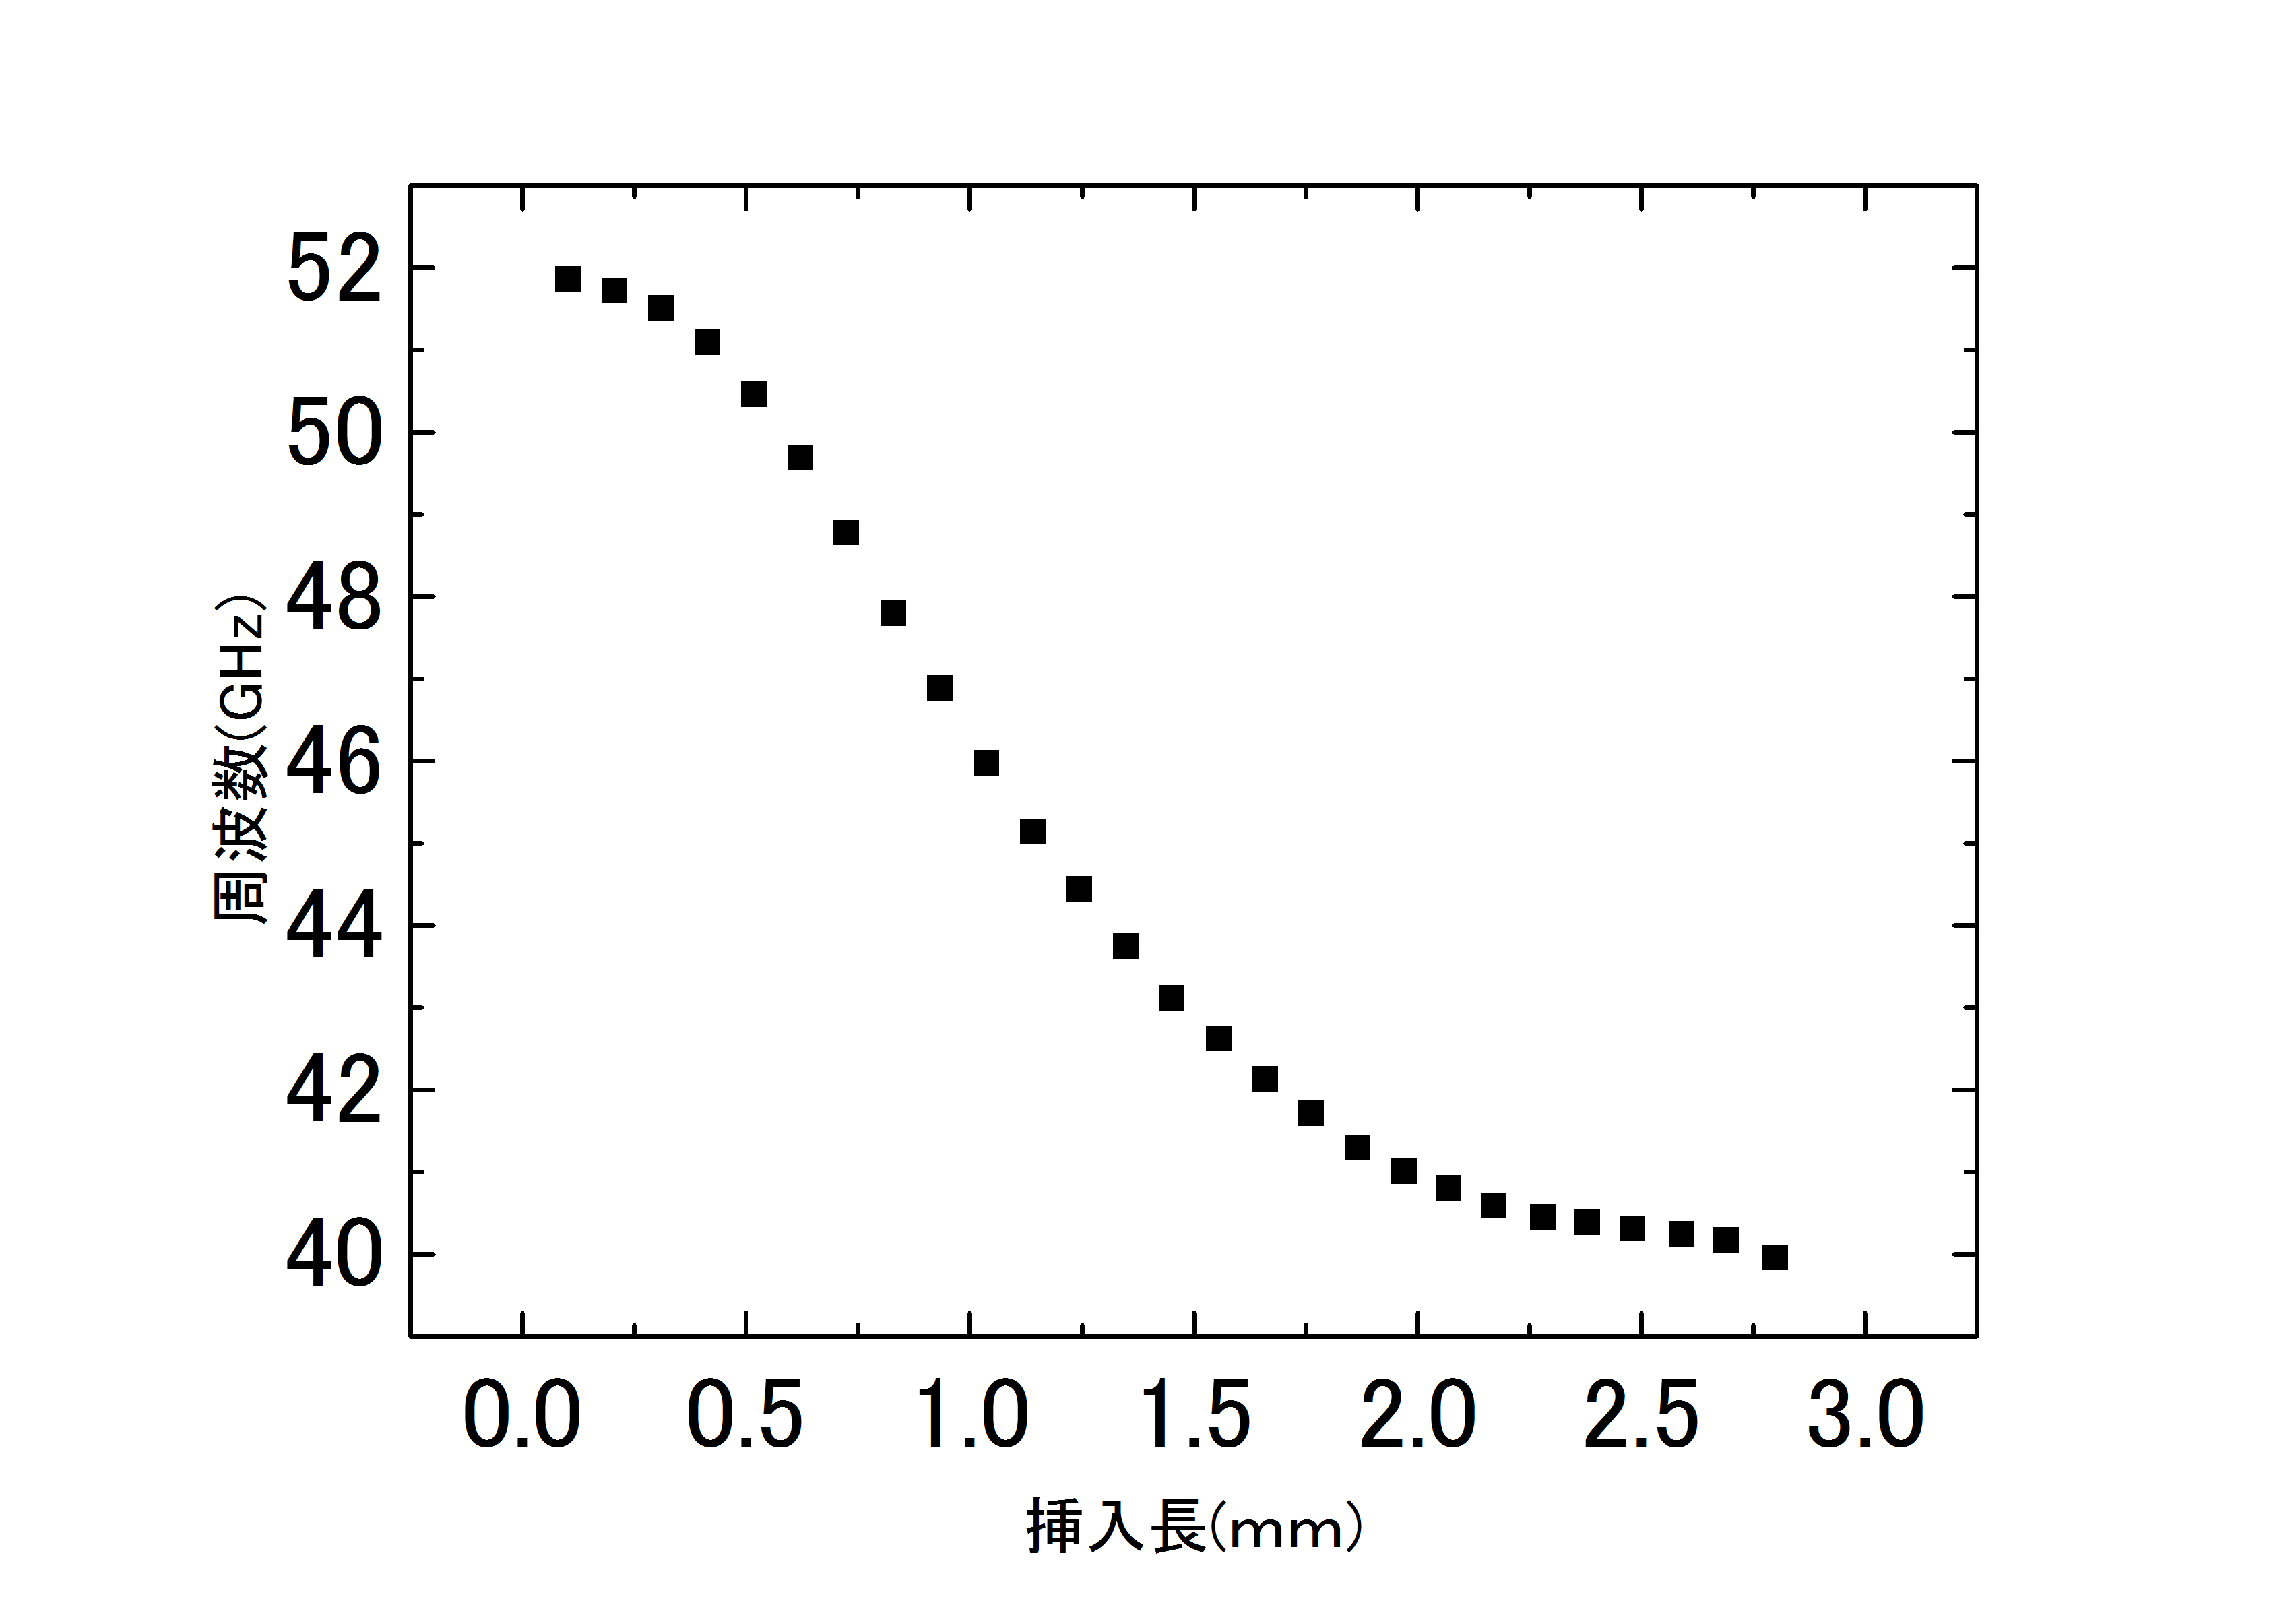
\includegraphics[width=12cm]{./image/plot2.jpg}
    \caption{誘電体挿入の際の共振周波数の変化}
    \label{fig:result}
  \end{center}
\end{figure}

この結果から、誘電体挿入に伴い、
40〜52GHz程度で共振周波数が変化する様子が観測できた。
また過渡解析の結果であるので、外界との電磁場結合ができており、
きちんと共振が起こるモデルであることがわかる。


% \subsection*{考察}
%
% あああああああああああああああ
% あああああああ
%
% あああああああ
% ああああ
%
% あああああああ
% ああああ
%
% あああああああああああああああ
% あああああああ
%
% あああああああああああああああ
% あああああああ
